    \item Consider a system of linear equations:
    \begin{align*}
        x-2y+3z &= -1, \\
        x-3y+4z &= 1,  \\
        -2x+4y-6z &= k
    \end{align*}
    The value of $k$ for which the system has infinitely many solutions is \underline{\hspace{2cm}}.

    \hfill{\brak{\text{EC 2015}}}
    \item The value of $p$ such that the vector $\myvec{1\\ 2\\ 3}$ is an eigenvector of the matrix $\myvec{4 & 1 & 2\\ p & 2 & 1\\ 14 & -4 & 10}$ is \underline{\hspace{2cm}}.
    \hfill{\brak{\text{EC 2015}}}
    \item In the given circuit, the values of $V_{1}$ and $V_{2}$ respectively are
    \hfill{\brak{\text{EC 2015}}}
    \begin{figure}[H]
        \centering
        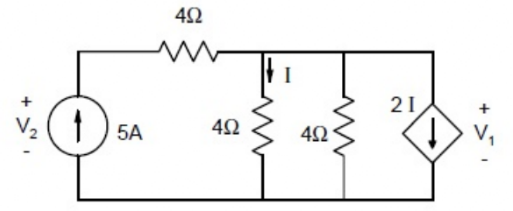
\includegraphics[width=0.5\columnwidth]{GATE/2015/EC/figs/q18.png}
        \caption*{}
        \label{fig:q18}
    \end{figure}
    \begin{enumerate}
        \begin{multicols}{4}
            \item 5 V, 25 V
            \item 10 V, 30 V
            \item 15 V, 35 V
            \item 0 V, 20 V
        \end{multicols}
    \end{enumerate}
    \item Two sequences $[a,b,c]$ and $[A,B,C]$ are related as,
    $$ \myvec{A\\ B\\ C} = \myvec{1 & 1 & 1\\ 1 & W_{3}^{-1} & W_{3}^{-2}\\ 1 & W_{3}^{-2} & W_{3}^{-4}} \myvec{a\\ b\\ c}$$ 
    where $W_{3}=e^{j\frac{2\pi}{3}}$. If another sequence $[p,q,r]$ is derived as,
    \[ \myvec{p\\ q\\ r} = \myvec{1 & 1 & 1\\ 1 & W_{3}^{1} & W_{3}^{2}\\ 1 & W_{3}^{2} & W_{3}^{4}} \myvec{1 & 0 & 0\\ 0 & W_{3}^{2} & 0\\ 0 & 0 & W_{3}^{4}} \myvec{A/3\\ B/3\\ C/3}, \]
    then the relationship between the sequences $[p,q,r]$ and $[a,b,c]$ is
    \hfill{\brak{\text{EC 2015}}}
        \begin{multicols}{2}
    \begin{enumerate}
        \item $[p,q,r]=[b,a,c]$
        \item $[p,q,r]=[b,c,a]$
        \item $[p,q,r]=[c,a,b]$
        \item $[p,q,r]=[c,b,a]$
    \end{enumerate}
\end{multicols}
    
